\documentclass{beamer}
\mode<presentation>
{
\usepackage{dis-template}
}
\usepackage{listings}
\usepackage{hyperref}
\usepackage{textcomp}
\definecolor{comments}{HTML}{50c878}
\lstset{language=C++,
  basicstyle=\ttfamily,
  keywordstyle=\color{blue}\ttfamily,
  stringstyle=\color{red}\ttfamily,
  commentstyle=\color{comments}\ttfamily,
  breaklines=true
}
\graphicspath{{slides/}} % TODO: eliminate this hack, necessary because scons builds at repository root

%---------------------------------------------------------------------
\titlepageinit{1}{Introduction}{21 Jan 2015 (Week 1)}
%---------------------------------------------------------------------
\begin{document}
%---------------------------------------------------------------------
\begin{frame}
\titlepage

\setcounter{tocdepth}{1}
\tableofcontents
\end{frame}

% LAB PREPARATION
% Distribute FRDM-KL25Z boards to all stations along with mini-USB cables
% Ensure resistors and LEDs are stocked

%---------------------------------------------------------------------
\section{Administrivia} % [5 mins]
%---------------------------------------------------------------------
\subsection{Getting Started...}

\begin{frame}
\frametitle{Welcome}
\begin{center}
{\huge Welcome to EE192!}
\end{center}
\end{frame}

\begin{frame}
\frametitle{Project}
\begin{columns}[t]
\column{0.646\textwidth}
\begin{itemize}
  \item Project: build an autonomous track-following racecar given a stock chassis and microcontroller dev kit
  \item Teams should be 3 students
  \begin{itemize}
    \item Combined skillset should include mechanical design / fabrication, electronics, programming
    \item Controls experience helpful
  \end{itemize}
  \item Teams formed by checkoff Friday
  \item Read the competition rules
  \begin{itemize}
    \item Freescale Cup
    \item NATCAR
  \end{itemize}
\end{itemize}

\column{0.323\textwidth}
\end{columns}
\end{frame}

\begin{frame}
\frametitle{Checkoffs}
\begin{columns}[t]
\column{0.646\textwidth}
\begin{itemize}
  \item One-hour time slot on Friday 11:30am-12:30pm to demonstrate that your project is where it should be
  \item At least one team member needs to show up to run your hardware
  \item These are graded, half credit if late
  \newline
  \item First checkoff this Friday
  \begin{itemize}
    \item Form project teams and check out cars
    \item Checks4Cars program: trade a \$300 deposit check for a car
    \item Get private course GitHub repository
    \item Details on website
  \end{itemize}
\end{itemize}

\column{0.323\textwidth}
\begin{figure}
\centering
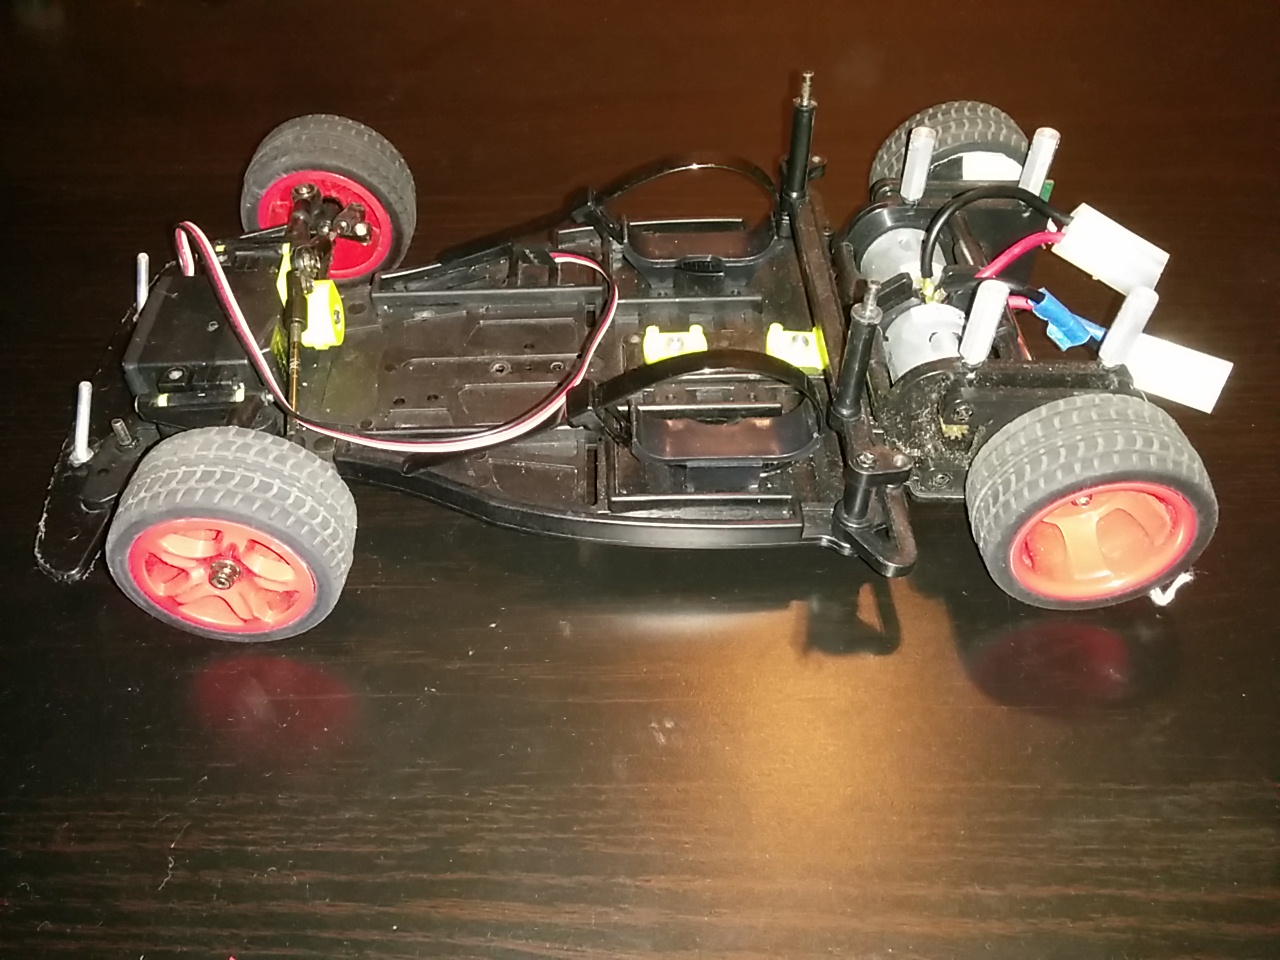
\includegraphics[width=1.0\columnwidth]{images-dis1/car-chassis}
\newline
Get your cars!
\end{figure}
\end{columns}
\end{frame}

\begin{frame}
\frametitle{Git Refresher}
\begin{columns}[t]
\column{0.646\textwidth}
\begin{itemize}
  \item Git: distributed version control software
  \begin{itemize}
    \item Each commit: like complete snapshot
    \item Branches: separate chains of commits
    \begin{itemize}
      \item eventually merged back to its parent
    \end{itemize}
    \item Distributed: everyone has compete copy
    \begin{itemize}
      \item Most operations local, periodically sync
    \end{itemize}
  \end{itemize}
  \item Best Practices
  \begin{itemize}
    \item Small, logical, often commits
    \item Write good commit messages
    \item Develop in branches: keep master clean
  \end{itemize}
\end{itemize}

\column{0.323\textwidth}
\begin{figure}
\centering

\includegraphics[width=1.0\columnwidth]{images-dis1/Git-Logo-2Color}
\newline
{\tiny git logo, by Jason Long, CC BY 3.0}\\
\vspace{20px}
Learn git here: \\
\url{try.github.io}

\end{figure}
\end{columns}
\end{frame}

%---------------------------------------------------------------------
\section{FRDM Board Intro} % [5 mins overview, 10 mins demo]
%---------------------------------------------------------------------
\subsection{Hardware}
\begin{frame}
\frametitle{Hardware}
\begin{columns}[t]
\column{0.646\textwidth}
\begin{itemize}
  \item FRDM-KL25Z Development Board
  \item MKL25Z128VLK4 microcontroller
  \begin{itemize}
    \item 48MHz ARM Cortex-M0+
    \item 128KB flash
    \item 16KB SRAM
  \end{itemize}
  \item Programmable using USB
  \item I/O headers including
  \begin{itemize}
    \item GPIO
    \item 16-bit analog inputs (ADC)
    \item 12-bit analog output (DAC)
    \item PWM, I\textsuperscript{2}C, SPI, and UART modules
  \end{itemize}
  \item On-board RGB LED and accelerometer
\end{itemize}

\column{0.323\textwidth}
\begin{figure}
\centering
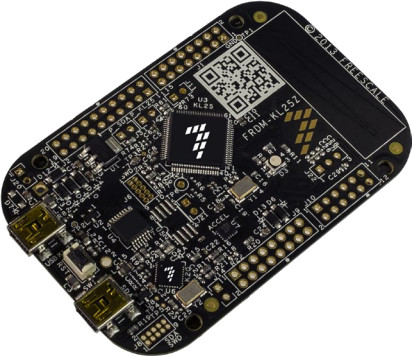
\includegraphics[width=1.0\columnwidth]{images-dis1/kl25z} \\
FRDM-KL25Z Board \\
{\tiny image from KL25Z User's Manual}
\end{figure}
\end{columns}
\end{frame}

%---------------------------------------------------------------------
\subsection{MCU Refresher}
\begin{frame}
\frametitle{IO Refresher}
\begin{columns}[t]
\column{0.646\textwidth}
\begin{itemize}
  \item GPIO (general purpose input/output) pins
  {\tiny\url{http://developer.mbed.org/handbook/DigitalOut}
    \url{http://developer.mbed.org/handbook/DigitalIn}}
  \begin{itemize}
    \item As an output: sets voltage on pin from software, either GND (0) or Vdd (1)
    \item As an input: samples voltage on the pin, returning either 0 (low) or 1 (high)
  \end{itemize}
  \item PWM (pulse-width modulation) module
  {\tiny\url{http://developer.mbed.org/handbook/PwmOut}}
  \begin{itemize}
    \item Every \textit{period}, the pin is high based on the \textit{duty cycle}, then low for the remainder
    \item Can digitally approximate analog outputs
  \end{itemize}
  \item Analog Inputs (ADC)
  {\tiny\url{http://developer.mbed.org/handbook/AnalogIn}}
  \begin{itemize}
    \item Converts a continuous analog voltage (0-3.3v) to a 16-bit (0-65535) quantity
  \end{itemize}
\end{itemize}

\column{0.323\textwidth}
\begin{figure}
\centering
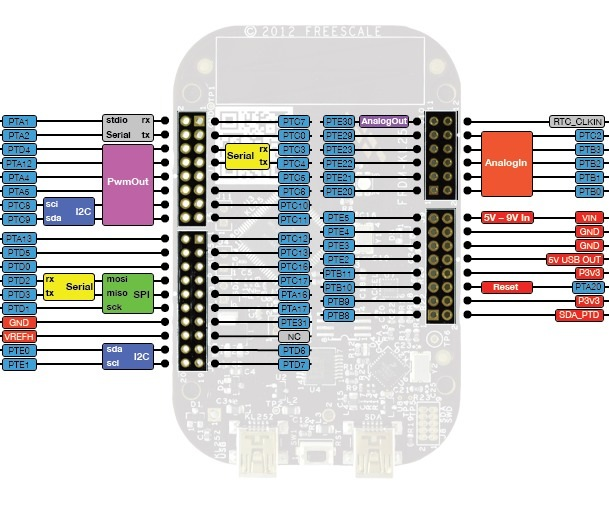
\includegraphics[width=1.0\columnwidth]{images-dis1/kl25z-pinout-revised}
\newline
FRDM-KL25Z pinout
{\tiny image from ???} % image was part of the Sp `14 checkpoint
% TODO: Perhaps add the board block diagram?
\end{figure}
\end{columns}
\end{frame}

\begin{frame}
\frametitle{Concurrency Refresher}
\begin{columns}[t]
\column{0.646\textwidth}
\begin{itemize}
  \item FRDM-KL25Z's processor is single core
  \item Blocking Operations
  \begin{itemize}
    \item Operations do not return until finished, blocking thread of control
    \item IO operations may be lengthy!
  \end{itemize}
  \item Nonblocking Operations
  \begin{itemize}
    \item Operations return immediately, activity continues in the ``background''
    \item IO operations can buffer data and use interrupts to send/receive data
  \end{itemize}
  \item Threading and RTOS \\
  \tiny{\url{http://developer.mbed.org/handbook/RTOS}}
  \begin{itemize}
    \item mBed has a RTOS with threading, concurrency, and synchronization
    \item Beware of threading anti-patterns
  \end{itemize}
\end{itemize}

\column{0.323\textwidth}
% TODO: Perhaps a threading diagram here?
\end{columns}
\end{frame}

\subsection{Skeleton Code}

\begin{frame}[fragile]
\frametitle{``Hello, World!'' Code}
\begin{columns}[t]
\column{0.55\textwidth}
\centering
\begin{lstlisting}[language=C++,basicstyle=\ttfamily\tiny]
MODSERIAL serial(USBTX, USBRX);

DigitalOut led_green(LED_GREEN);
DigitalOut led_red(LED_RED);
PwmOut led_blue(LED_BLUE);

int main() {
  // Internal LED is active low.
  led_green = 0;  
  wait(0.25);
  led_green = 1;
  wait(0.25);
  
  // Mandatory "Hello, world!".
  serial.printf("Hello, world!\r\n");

  // Run led_fade_thread() in own thread
  Thread ledFadeThread(led_fade_thread);
  
  // Periodically call led_blink_periodic()
  RtosTimer ledBlinkTimer(led_blink_periodic);
  ledBlinkTimer.start(1000);

  // Work is done in the threads,
  // so main() can sleep.
  Thread::wait(osWaitForever);
}
\end{lstlisting}

\column{0.45\textwidth}
\begin{lstlisting}[language=C++,basicstyle=\ttfamily\tiny]
void led_fade_thread(
    void const *args) {
  // Note this doesn't temrinate.
  while (1) {
    // Invert duty cycle.
    led_blue.write(1-0);
    Thread::wait(250);
    led_blue.write(1-0.25);
    Thread::wait(250);
    led_blue.write(1-0.5);
    Thread::wait(250);
    led_blue.write(1-0.75);
    Thread::wait(250);
  }
}

void led_blink_periodic(
    void const *args) {
  // Toggle the red LED when called.
  led_red = !led_red;
}
\end{lstlisting}
\end{columns}
\end{frame}

\begin{frame}
\frametitle{Hello, World! Demo}
\begin{center}
{\huge Live Demo!} \\
\vspace{20px}
\tiny{This is essentially the procedure demonstrated in the checkpoint 1 page} \\
\vspace{20px}
\tiny{... and hopefully goes Murphy-free ...} \\
\vspace{40px}
{\tiny Note: you'll have to download the Device Family Pack for the FRDM-KL25Z \\
\url{http://www.keil.com/dd2/arm/armcm0/} \\
(also on the checkpoint page)} \\
\end{center}
\end{frame}

%---------------------------------------------------------------------
\section{Soldering} % [10 mins overview, remainder lab]
%---------------------------------------------------------------------
\subsection{Theory}
\begin{frame}
\frametitle{Overview}
% Soldering theory
%% PTH and SMT overview - we focus on PTH
\begin{columns}[t]
\column{0.646\textwidth}
\begin{itemize}
  \item Soldering: joining (electrically and mechanically) metals using a separate fillter metal ``\textit{solder}''
  \item Electronics: bonding component pins/leads to circuit board through-holes or pads
  \begin{itemize}
    \item Solder is usually a tin/lead alloy (e.g. 63/37) or lead-free tin-silver-copper alloy (e.g. SAC305)
  \end{itemize}
  \item This tutorial focuses on introductory through-hole soldering
  \begin{itemize}
    \item Note: most production boards today are surface-mount to save space
  \end{itemize}
\end{itemize}

\column{0.323\textwidth}
\begin{figure}
\centering
Example solder joints: \\
\vspace{20px}
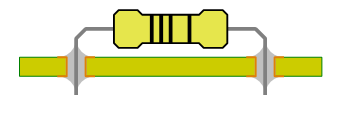
\includegraphics[width=1.0\columnwidth]{images-dis1/pcb-pth} \\
Through-hole \\
\vspace{20px}
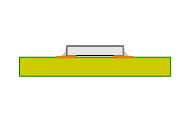
\includegraphics[width=1.0\columnwidth]{images-dis1/pcb-smt} \\
Surface-mount
\end{figure}
\end{columns}
\end{frame}

\begin{frame}
\frametitle{Safety Precautions}
%% What is soldering, safety precautions (lead, flux fumes, things get HOT, flux splatter: goggles)
%% Board Delamination
\begin{columns}[t]
\column{0.646\textwidth}
\begin{itemize}
  \item Soldering melts metal - IT'S HOT
  \begin{itemize}
    \item Tips typically set at 700\textdegree F (371\textdegree C)
    \item Irons can stay hot after turning off
    \item Touching a hot tip is NOT fun
  \end{itemize}
  \item Leaded solder contains, well, lead...
  \begin{itemize}
    \item ... which is known to the state of California to cause cancer and reproductive harm ...
    \item WASH YOUR HANDS AFTERWARDS
  \end{itemize}
  \item Solder vaporizes flux, producing fumes
  \begin{itemize}
    \item Regular exposure linked to asthma
    \item DON'T BREATHE THEM IN
    \item May also cause solder splatter: \\
    safety goggles recommended
  \end{itemize}
\end{itemize}

\column{0.323\textwidth}
\begin{figure}
\centering

\includegraphics[width=0.8\columnwidth]{images-dis1/house}
\newline
Lead poisoning: \\
not as fun in real life
{\tiny \textcopyright Fox}
\end{figure}
\end{columns}
\end{frame}

\begin{frame}
\frametitle{Oxidation}
%% High temperature chemical processes, oxidation and flux
%% Board Delamination
\begin{columns}[t]
\column{0.646\textwidth}
\begin{itemize}
  \item Soldering depends on good thermal transfer from tip to solder / component / board
  \item Metals oxidize, forming an oxide layer
  \begin{itemize}
    \item Oxides impede thermal transfer
    \item Reactions faster at higher temperatures
  \end{itemize}
  \item Flux provides chemical cleaning
  \begin{itemize}
    \item Rosin flux is corrosive when heated
    \item ... and is present in solder wire spools
    \item ... but is ``burned'' upon use
  \end{itemize}
  \item Just keep this in mind...
\end{itemize}

\column{0.323\textwidth}
\begin{figure}
\centering
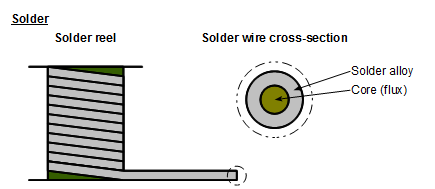
\includegraphics[width=1.0\columnwidth]{images-dis1/solder-reel}
\newline
Solder cross-section \\
showing flux core
\end{figure}
\end{columns}
\end{frame}

\begin{frame}
\frametitle{Equipment Overview}
\begin{figure}
\centering
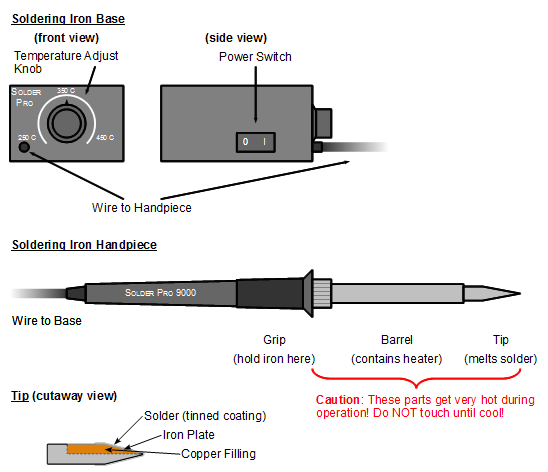
\includegraphics[width=\textwidth,height=0.8\textheight,keepaspectratio]{images-dis1/solder-station}
\end{figure}
\end{frame}

%---------------------------------------------------------------------
\subsection{Procedure}
\begin{frame}
\frametitle{Tip Maintenence}
%% Cleaning / tinning the tip / theory (fresh solder for heat transfer) / why this needs do be done often / why to keep tip tinned
\begin{columns}[t]
\column{0.646\textwidth}
\begin{itemize}
  \item The tip is what heats things up
  \begin{itemize}
    \item Want to maximize thermal transfer!
  \end{itemize}
  \item Keep the tip ``tinned'' with solder
  \begin{itemize}
    \item Provides better thermal transfer
    \item Sacrificial layer preventing tip oxidation, \\
    which destroys the tip
  \end{itemize}
  \item Must be occasionally refreshed
  \begin{itemize}
    \item The solder oxidizes, accelerated by heat
    \item Cleaning: wipe on brass or wet sponge
    \item Immediately re-tin (apply solder layer)
  \end{itemize}
\end{itemize}

\column{0.323\textwidth}
\begin{figure}
\centering
% TODO: Add some useful graphic here, like expanded tip graphic
\end{figure}
\end{columns}
\end{frame}

\begin{frame}
\frametitle{Procedure}
%% Maximizing heat transfer: soldering with broad end / chisel tip
%% Process per lead / rinse and repeat
\begin{itemize}
  \item Beginner's tip: use iron to heat up component and board, not solder
  \begin{itemize}
    \item Feed solder in through the other side
    \item Solder only melts when component and board sufficiently hot
  \end{itemize}
  \item Maximizing heat transfer
  \begin{itemize}
    \item Point tips: solder using ``side'' of tip, not point
    \item Chisel tips: use the broad flat end
  \end{itemize}
\end{itemize}
\begin{figure}
\centering
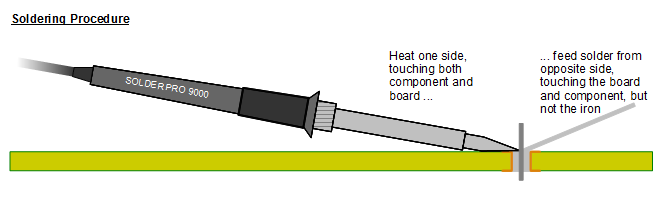
\includegraphics[width=0.8\textwidth,height=0.8\textheight,keepaspectratio]{images-dis1/solder-pth-technique}
\end{figure}
\end{frame}

\begin{frame}
\frametitle{Joint Inspection}
Optimal joint shape is a ``solder volcano''
\begin{figure}
\centering
% TODO: split into several graphics
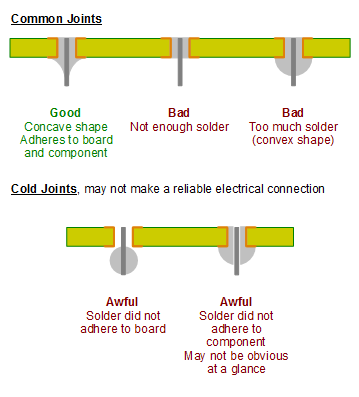
\includegraphics[width=\textwidth,height=0.8\textheight,keepaspectratio]{images-dis1/solder-joints}
\end{figure}
\end{frame}

%---------------------------------------------------------------------
\subsection{Lab}
\begin{frame}
\frametitle{Through-Hole Soldering Demo}
\begin{center}
{\huge Live Demo!} \\
\vspace{20px}
{\tiny... which REALLY hopefully goes Murphy-free ...}
\end{center}
\end{frame}

\begin{frame}
\frametitle{Scheduling}
\begin{columns}[t]
\column{0.646\textwidth}
\begin{itemize}
  \item Quick poll: best time for GSI office hours? \\
  (about 2 per week)
  \begin{itemize}
    \item Thursday, for the pre-checkoff scramble?
    \item Other times?
  \end{itemize}
  \item Thursday section only: has schedules cleared up enough to move discussion to Wednesday?
  \begin{itemize}
    \item Otherwise, future discussion sections (starting Thu, 29 Jan) will be 9:30am-10:30am
  \end{itemize}
\end{itemize}

\column{0.323\textwidth}
\end{columns}
\end{frame}

\begin{frame}
\frametitle{Electrostatic Discharge}
\begin{columns}[t]
\column{0.646\textwidth}
\begin{itemize}
  \item You build up static charge on your body
  \begin{itemize}
    \item ... just by walking, especially when it's dry
    \item ... and up to several kV
    \item but under $\sim$2kV is imperceptible
  \end{itemize}
  \item Chips are sensitive to high voltages: \\
  \textbf{may cause permanent damage}
  \begin{itemize}
    \item read: board stops working ``for no reason''
  \end{itemize}
  \item Remember to ground (discharge) yourself before handling sensitive electronics
  \begin{itemize}
    \item Touch the grounded lab bench surface
    \item Use a ESD wriststrap
    \item Avoid touching traces on boards
  \end{itemize}
\end{itemize}

\column{0.323\textwidth}
\begin{figure}
\centering
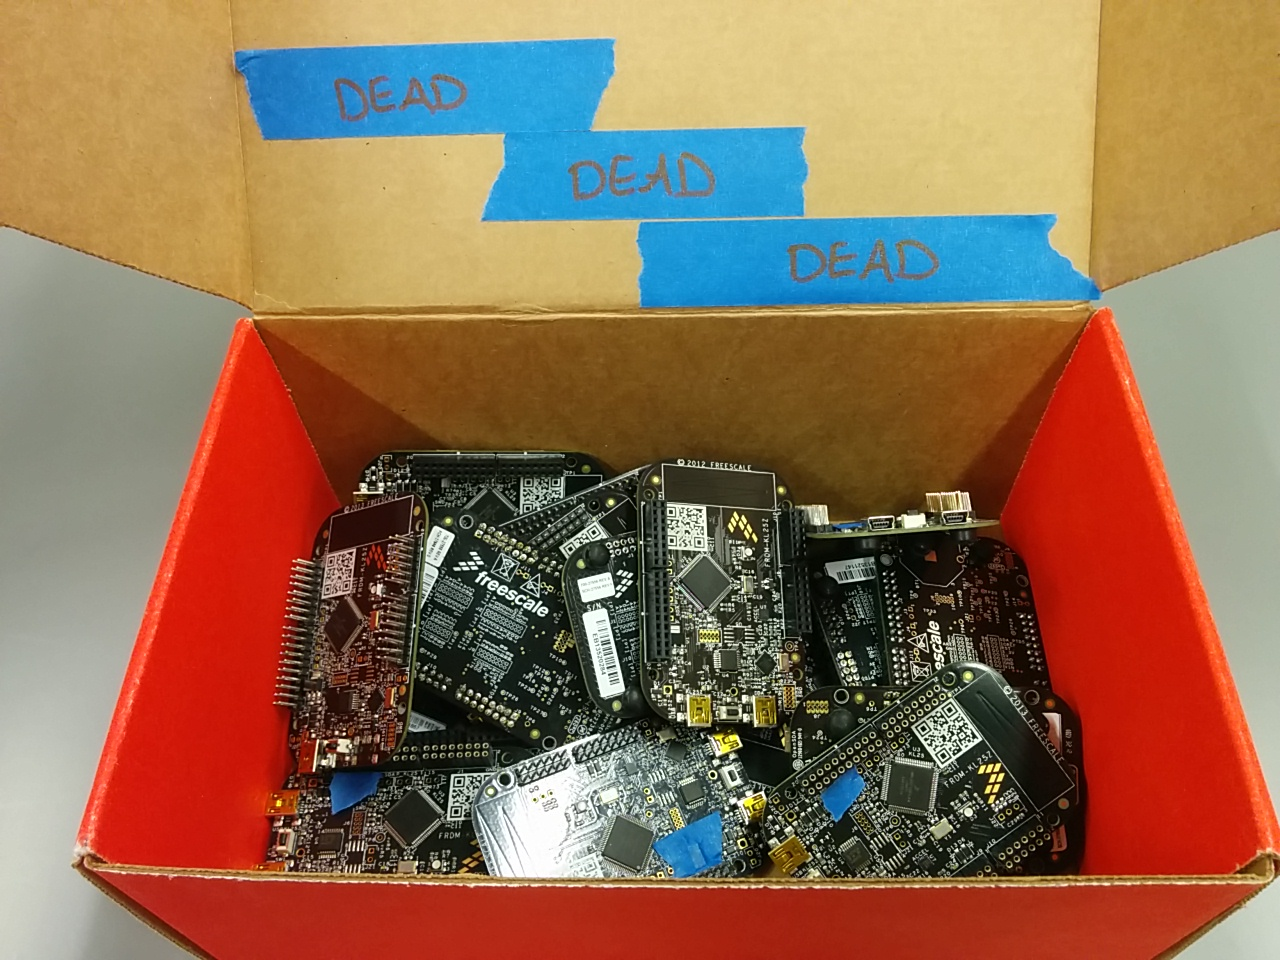
\includegraphics[width=0.8\columnwidth]{images-dis1/fried-boards}
\newline
Don't let this happen \\
to you
\end{figure}
\end{columns}
\end{frame}

\begin{frame}
\frametitle{Fin}
\begin{center}
Get your parts and get started! \\
\vspace{5px}
{\tiny I'll be walking around helping!} \\
\vspace{20px}
For checkpoint 1, you need to solder a resistor and LED onto perfboard \\
Choose the resistor such that $\sim$1.6mA goes through the LED \\
The MCU supply voltage is 3.3v \\
\vspace{5px}
{\tiny (yes, I know those red LEDs suck)} \\
\vspace{20px}
Also, grab a computer account form!
\end{center}
\end{frame}


\end{document}
